\chapter{Outras informações}
	Para estudar como passar a ideia da máquina de estado para um código em
	Verilog, pensou-se numa máquina simples, que tem como estado inicial o estado A,
	que vai para um estado B e o B vai para o A. Assim, para determinar em que estado
	a máquina encontra-se, estipulou-se \ac{led}s para representar o estado atual,
	\ac{led} verde para o estado A e para B um \ac{led} vermelho.

	O desenho da máquina encontra-se na \autoref{figura:adicional},
	o Verilog no \autoref{codigo:adicional}, a compilação na
	\autoref{figura:compilacaoAdicional}, código do teste
	no \autoref{codigo:testBenchAdicional} e os testes nas
	\autoref{figura:testBenchWaveAdicional} e \autoref{figura:testBenchTranscriptAdicional}.

	\begin{figure}[H]
		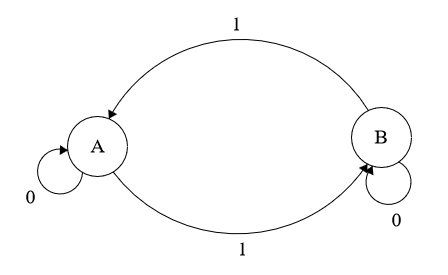
\includegraphics{img/maquinaAdicional/maquinaEstado}
		\caption{Máquina de estado do circuito adicional.}
		\label{figura:adicional}
	\end{figure}

	\lstinputlisting[label = {codigo:adicional},caption = {Código da máquina de estado adicional.}]
	{codigo/circuitoAdicional.v}

	\begin{figure}[H]
		\centering
		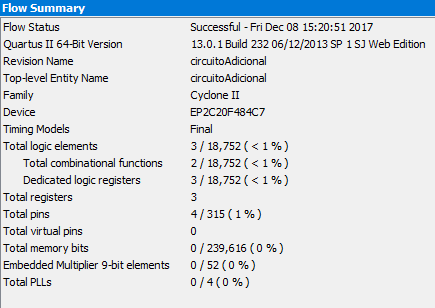
\includegraphics[width=0.4\textwidth]{img/maquinaAdicional/compilacao}
		\caption{Compilação da máquina de estado do circuito adicional.}
		\label{figura:compilacaoAdicional}
	\end{figure}

	\lstinputlisting[label = {codigo:testBenchAdicional},caption = {Código do \textit{test bench} da máquina de estado adicional.}]
	{codigo/circuitoAdicional_TB.v}

	\begin{figure}[H]
		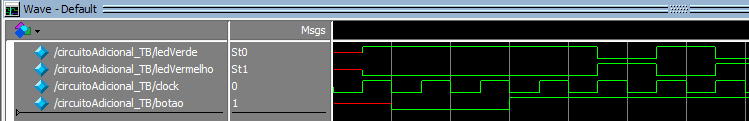
\includegraphics[width=1\textwidth]{img/maquinaAdicional/testBenchWave}
		\caption{\textit{Test bench Wave} da máquina de estado adicional.}
		\label{figura:testBenchWaveAdicional}
	\end{figure}

	\begin{figure}[H]
		\centering
		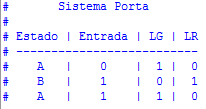
\includegraphics{img/maquinaAdicional/testBenchTranscript}
		\caption{\textit{Test bench Transcript} da máquina de estado adicional.}
		\label{figura:testBenchTranscriptAdicional}
	\end{figure}
